%!TEX root = ../../super_main.tex

\section{Providing Sensor Data}
\label{sec:providing_sensor_data}

We have designed a general abstraction, called a \emph{Sensor Provider}, for the different available sensors to support the structure of the data described in \secref{sec:temporal_properties_of_snapshots}. This abstraction is designed for concurrent and independent collection of samples, as we want the application to be able to gather information from multiple sources at the same time. This means that the system is able to, for instance, collect data regarding the motion and location of the participant simultaneously. This is done to ensure that the gathered data is obtained according to the desired temporal properties, i.e. the time constraints of snapshots as seen in \figref{fig:sample_temporality}.

%As described in \secref{sec:deriving_the_context_from_sensors}, there exist various types of sensors, each outputting measurements in various formats. 

\subsection{Caching Sensor Values}
\label{sub:caching_sensor_values}
On the Android platform, some sensors are of an reactive nature (see \secref{sec:deriving_the_context_from_sensors}), meaning that events will raised whenever a sensor fluctuates. For instance, the accelerometer sensor in an Android device only raises events, whenever the device is affected in some way, meaning that events may never be raised if the phone is laying completely still. This causes problems with the temporal properties described in \secref{sec:temporal_properties_of_snapshots}, because it is impossible to know when these events will trigger, and we want to guarantee that measurements can be made with a specific frequency. For sensors of this nature, we need to somehow cache the values that the sensor returns during these event, such that we can utilize them when needed. To solve this problem we introduce a cache for each sensor that will be updated each time such an event occurs for the given sensor.
\\\\
The idea is then that sensor updates can happen completely asynchronously, independent from the rest of the system, meaning that acquisition of the most recent reading can happen synchronously. \figref{fig:cache_examples} shows how this independent behavior provides an interface for a time driven process that wants to acquire measurements synchronously, without worrying about the events of individual sensors. \figref{fig:cache_no_event_between} shows a scenario where some other process requests a measurement multiple times, and where the events from the sensors are not triggered in between. This process will, as shown, be answered with the same measurement in both of its requests. The cached measurement is however still correct, because the underlying sensor has not registered a change and raise an event in the given time frame. Another scenario is shown in \figref{fig:cache_multiple_event_between}, where multiple events are triggered between two measurement requests from another process. The interface is also sound here because the most recent measurement, with the desired frequency, is returned.

\begin{figure}[!htbp]
\begin{subfigure}[!t]{.5\textwidth}
  \centering
  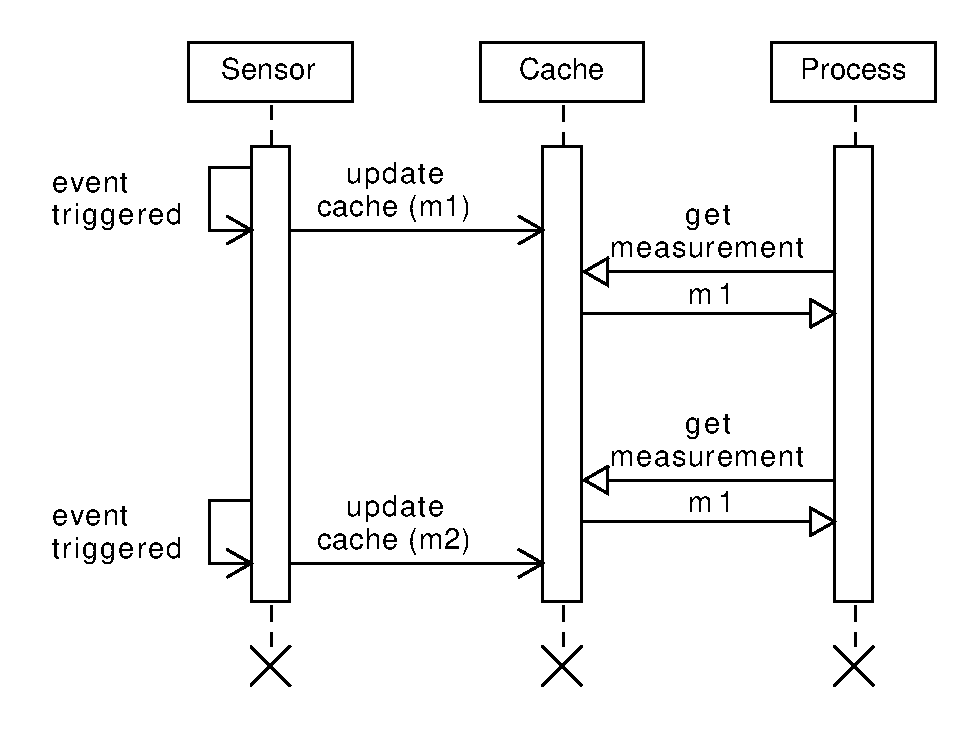
\includegraphics[width=\linewidth]{sensor_providers/cache_example_1}
  \caption{No events between requests.}
  \label{fig:cache_no_event_between}
\end{subfigure}
\begin{subfigure}[!t]{.5\textwidth}
  \centering
  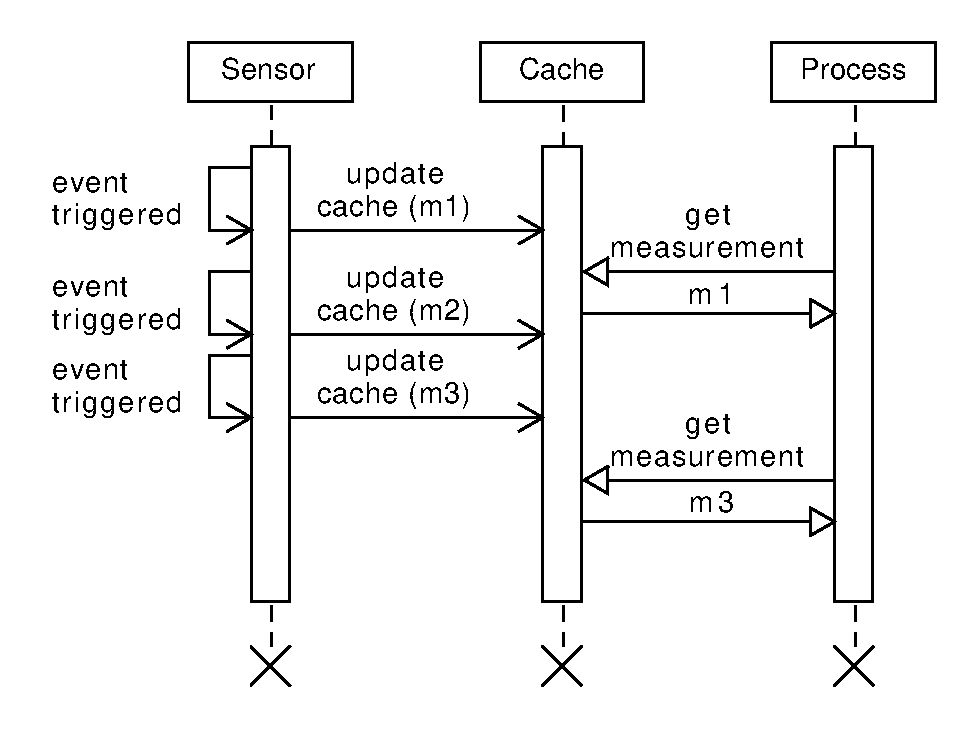
\includegraphics[width=\linewidth]{sensor_providers/cache_example_2}
  \caption{Multiple events between requests.}
  \label{fig:cache_multiple_event_between}
\end{subfigure}
\caption{Measurement caching.}
\label{fig:cache_examples}
\end{figure}
\FloatBarrier

One issue this design might introduce is that we rely on these sensor events being raised eventually. The cache must contain some default value for a sensor, if this is not the case, which could potentially pollute the measurements until the first event is triggered. This means that until the first event is raised other processes will be answered with default values. However, since the default values from sensors are distinguishable from actual measurements, this should not be a problem for customers.

%Other types of data sources, which are not event driven, such as Wi-Fi, are, as mentioned in \secref{sec:deriving_the_context_from_sensors}, available on demand meaning that we are able to acquire the access point data at any given time as long as Wi-Fi is enabled, meaning that some data sources already provide the desired behavior. Some of these on demand sensors might take some time to acquire the information. An example of this could be triangulation based on satellites for GPS. A potential problem here, in regards to timing, is therefore latency before the underlying system is ready to return the data to the caller. This effectively means that the first few measurements for some of the sensors will not reflect the reality they measure, since they have not taken any measurements yet.

\subsection{Sensor Providers}
\label{sub:providing_sensor_data_implementation}
We have implemented our \emph{Sensor Provider} as an abstract class, called \mono{SensorProvider}, which must be subclassed for each type of available sensor, both for sensors found on the actual Android devices which runs the application, but also for sensors in connected wearables, such as those found in a Microsoft Band 2. The abstract class provides functionality that makes it easy to implement specialized implementations for every sensor that we have. Sub-classes of the abstract \mono{SensorProider}, must specify a type argument, \mono{MeasurementT}, describing the type of the measurements which the implementation will make. Based on this measurement type, the super class can implement a method called \mono{onNewMeasurement(MeasurementT)}, which specializations must call in order to update the cache described in \secref{sub:caching_sensor_values}. Besides this, the following methods must be implemented by specializations:

\begin{description}
	\item[\mono{boolean isSensorAvailable()}] should return \mono{true}, if the sensor is currently available and ready to make measurements. It should return \mono{false}, if the sensor is unavailable or not present on the device. Overriding this method should be simple for most built-in sensors, which are always available if they are included in a device. It should be sufficient with a simple system call, to check if the sensor is present in the device. Overriding the method for other data sources such as Wi-Fi might prove more complicated, because the physical presence of a Wi-Fi radio in the device does not imply that the radio is turned on and active.

	\item[\mono{SensorType getSensorType()}] should return the type of sensor the provider is making available. The return type is an enum called \mono{SensorType}, allowing us to differentiate between the different sensor providers.

	\item[\mono{EventListenerRegistrationManager createRegManager()}] should return an instance of a class that implements the \mono{EventListenerRegistrationManager} interface. This interface will enforce the class to implement the following two methods: \mono{void register(int frequency)} and \mono{void unregister()}, which will be called by the super class to, for instance, register and unregister an event listener that will call \mono{onNewMeasurement(MeasurementT)} when events are raised.

  \item[\mono{MeasurementT getDefaultMeasurement()}] should return an object of the type \mono{MeasurementT}, for instance \mono{FloatMeasurement}. This object should represent the default value for that particular sensor. This value will be used when the sensor cache has not yet been set. It should be trivial to see if this measurement is a default value, so that customers can handle, or ignore, these measurements when processing the data.
\end{description} 

\todo[inline]{LÆS HERFRA}
In implementing the abstract methods for a given sensor in a specialization of \mono{Sensor\-Provider}, the super class will be able to produce a list of samples. The generation of the list of samples is done by utilizing two timed tasks. One that will be run every time a sample is due, until the total duration of a snapshot has passed. In this task, the second timed task is started. The job of the second task is to collect the individual measurements and join them into a sample. This is then collected and returned to the outer timed task, which will bundle these, and deliver them to the original caller as a list of samples. 
\\\\
The generation will start when the method, \mono{Future<List<Sample>> retrieve\-Samples\-For\-Duration()}, is called. The method takes the temporal properties, as covered in \secref{sec:temporal_properties_of_snapshots} and shown in \figref{fig:sample_temporality}, as parameters in order to give the timed tasks the wanted behavior. The return type of the method is a \mono{Future} object, which encapsulates the list of samples. A \mono{Future} object works as a handle on the result of an asynchronous task, meaning that it might or might not have the result when the method returns. Once the result of the \mono{Future} is needed one can call the \mono{get()} method on the object, which will block the caller until the result is ready. Using a \mono{Future} in this way allows us to start generation of the list of samples for different \emph{SensorProvider}s without having to wait for the result. It is then possible for us parallelize the collection of samples from sensors, and wait for them all simultaneously when needed. % With these measurements registered, the \mono{SensorProvider}, and in effect all of the sub-classes, are now able to construct \mono{Sample} objects by reading measurements from the cache with specific intervals.
\todo[inline]{LÆS HERTIL}

\subsubsection{Implementing a Sensor Provider}
Because of the abstract \mono{SensorProvider} class, new sensors can be implemented into the system with very few lines of code. An example of such an implementation can be seen in \lstref{lst:sensor_provider_acclerometer}, which shows the \emph{full} implementation of how the \mono{AccelerometerSensorProvider}. We have, as seen in \lineref{line:sensor_provider_extends}, subclassed \mono{SensorProvider} with the generic parameter \mono{FloatTripleMeasurement}, which is the output type for the accelerometer sensor. Furthermore, we have overridden the abstract methods: 

\begin{description}
  \item[\mono{boolean isSensorAvailable()}] is overridden in \linesref{line:isSensorAvailable_start}{line:isSensorAvailable_end}. Here we check if the phone has the system feature \mono{FEATURE\_SENSOR\_ACCELEROMETER}, if this is the case, we are able to measure accelerometer.

  \item[\mono{SensorType getSensorType()}] is overridden in \linesref{line:getSensorType_start}{line:getSensorType_end}. This method simply returns the enum value \mono{SensorType.ACCELEROMETER}.

  \item[\mono{EventListenerRegistrationManager createRegManager()}] is overridden in \linesref{line:createRegManager_start}{line:createRegManager_end} and will first construct a listener, registering new measurements whenever the sensor outputs new values. We do not wish to do anything when the accuracy of the sensor changes, so this block is empty. Lastly, we create the registration manager, based on fields found on the \mono{SensorProvider} class, and the listener we created.

  \item[\mono{FloatTripleMeasurement getDefaultMeasurement()}] is overridden in \linesref{line:getDefaultMeasurement_start}{line:getDefaultMeasurement_end}, simply returning a new \mono{FloatTripleMeasurement} instance with no values provided, causing the values to be initialized to \mono{0.0f}.
\end{description}

\lstinputlisting[
   style = Java,
   caption = {Implementation of sensor provider for the accelerometer sensor.},
   label = {lst:sensor_provider_acclerometer},
   float=!htbp,
]{content/gathering_sensor_data/code_snippets/sensor_provider_acclerometer.java}
\FloatBarrier

\subsection{Gathering Data from the Microsoft Band 2}
Due to the structure of sensor providers, as described in \secref{sub:providing_sensor_data_implementation}, it is relatively easy to implement functionality that will gather information from the Microsoft Band 2 smart band. The only major difference between the sensors from this device, and the sensors in an Android smartphone, is that a connection between the smart band and the phone has to be made. This connection has to be available in all of the band sensor providers, thus we implemented an abstract class called \mono{SensorProviderBand}, extending \mono{SensorProvider}, which furthermore, implements the method \mono{getConnectedBandClient()}. This method will try to establish a connection to the smart band through the required Microsoft Health application\footnote{https://www.microsoft.com/microsoft-health/en-us}. The method can be seen in \lstref{lst:get_connected_band_client}. The method returns a boolean, indicating if the connection were established or not. Currently, connection failures are not handled, instead we simply try again at a later point in time when the connection is needed again. \mono{getConnectedBandClient()} assumes that only a single band is connected, even though the Microsoft Band 2 supports multiple devices, and thus only uses the first items of the \mono{devices} array \lineref{line:device_array_zero_index}. We have added some logging statements, compared to the original source, in order to ease debugging, see for instance \lineref{line:debug_log}. 

\lstinputlisting[
   style = Java,
   caption = {Establishing a connection between the Android application and the Microsoft Band 2. Code is based on Example Code by Joshua Drew Sr\protect\footnotemark},
   label = {lst:get_connected_band_client},
   float=!htbp,
]{content/gathering_sensor_data/code_snippets/get_connected_band_client.java}
\footnotetext{https://github.com/jdruid/Microsoft-Band-Heart-Rate-Demo-Android/}
\FloatBarrier

% \subsection{Asynchronous Delivery of Samples}
% A \mono{SensorProvider} subclass is, with the requirements implemented, able to provide a list of \mono{Sample} instances at some point in the future through a call to a member function on the abstract \mono{SensorProvider} class. This is captured by letting the method return an instance of \mono{Future<List<Sample>\mono{}>}. A \mono{Future} object is a reference to some other object which represents the result of some computation being performed on another thread. A client of \mono{SensorProvider} instances can the request multiple of such \mono{Future} instances and then, once having all the desired \mono{Future} instances, choose to synchronously call a \mono{get()} on the \mono{Future} instances and effectively wait for each of the asynchronous computations to complete.
% \\\\
% Using futures and not saving any intermediary state persistently might prove to be a problem for Snapshots which are configured to collect data for longer periods of time as they might quickly fill up the memory because the objects referenced by the \mono{Future} instances is not dereferenced, and thereby freed, before the tasks behind the \mono{Future} instances are completed. Further development on how to minimize memory consumption for Snapshot collection should be pursued.
